\documentclass{report}
\usepackage[margin=1in]{geometry} 
\usepackage{amsmath,amsthm,amssymb,amsfonts}
\usepackage{tabto}
\usepackage[yyyymmdd]{datetime}		% Date Formatting
\renewcommand{\dateseparator}{--}	% Date Formatting
\usepackage{arydshln} 				% \hdashline and \cdashline
\newcommand*{\tempb}{\multicolumn{1}{:c}{}} % Used for block matrices

% For clickable TOC
\usepackage{hyperref}
\hypersetup{
	colorlinks,
	citecolor=black,
	filecolor=black,
	linkcolor=black,
	urlcolor=black
}

% Custom Section Types
\theoremstyle{plain} % italics
\newtheorem*{thrm}{Theorem}
\newtheorem*{lemma}{Lemma}
\theoremstyle{definition} % normal type
\newtheorem*{ex}{Example}
\newtheorem*{defn}{Definition}
\newtheorem*{result}{Result}
\theoremstyle{plain} % italics

% For circled text
\usepackage{tikz}
\newcommand*\circled[1]{\tikz[baseline=(char.base)]{
            \node[shape=circle,draw,inner sep=0.8pt] (char) {#1};}}

% For equation system alignment
\usepackage{systeme,mathtools}
% Usage:
%	\[
%	\sysdelim.\}\systeme{
%	3z +y = 10,
%	x + y +  z = 6,
%	3y - z = 13}

\newenvironment{problem}[2][Problem]{\begin{trivlist}
\item[\hskip \labelsep {\bfseries #1}\hskip \labelsep {\bfseries #2.}]}{\end{trivlist}}
%If you want to title your bold things something different just make another thing exactly like this but replace "problem" with the name of the thing you want, like theorem or lemma or whatever
 
%used for matrix vertical line
\makeatletter
\renewcommand*\env@matrix[1][*\c@MaxMatrixCols c]{%
  \hskip -\arraycolsep
  \let\@ifnextchar\new@ifnextchar
  \array{#1}}
\makeatother 
 
% Change chapter numbering
\newcommand{\mychapter}[2]{
	\setcounter{chapter}{#1}
	\setcounter{section}{0}
	\chapter*{#2}
	\addcontentsline{toc}{chapter}{#2}
}

\title{CNN Report}
\author{Bryan Greener}
\date{2018-06-14}

\graphicspath{{./images/}}

\begin{document}
% BUILD TOC
%\tableofcontents{}
\maketitle
\section{Implementation}
In this assignment, I used Keras with Tensorflow as a backend to implement a Convolutional Neural Network for classifying MNIST, CIFAR-10, and the CIFAR-100 datasets. Choosing Keras helped to simplify the structure of the code in a way that made it much easier to learn as opposed to just using Tensorflow. Each of the datasets used had a very similar network structure however when using larger datasets such as CIFAR-10 and CIFAR-100, a few changes to the types and numbers of layers in the network needed to take place.
\subsection{MNIST}
For the MNIST dataset, I used two convolutional/pooling layers followed by two fully connected layers. Since there is only one color channel due to these images being black and white, then the input layer only has a single channel as well.
\begin{figure}[h]
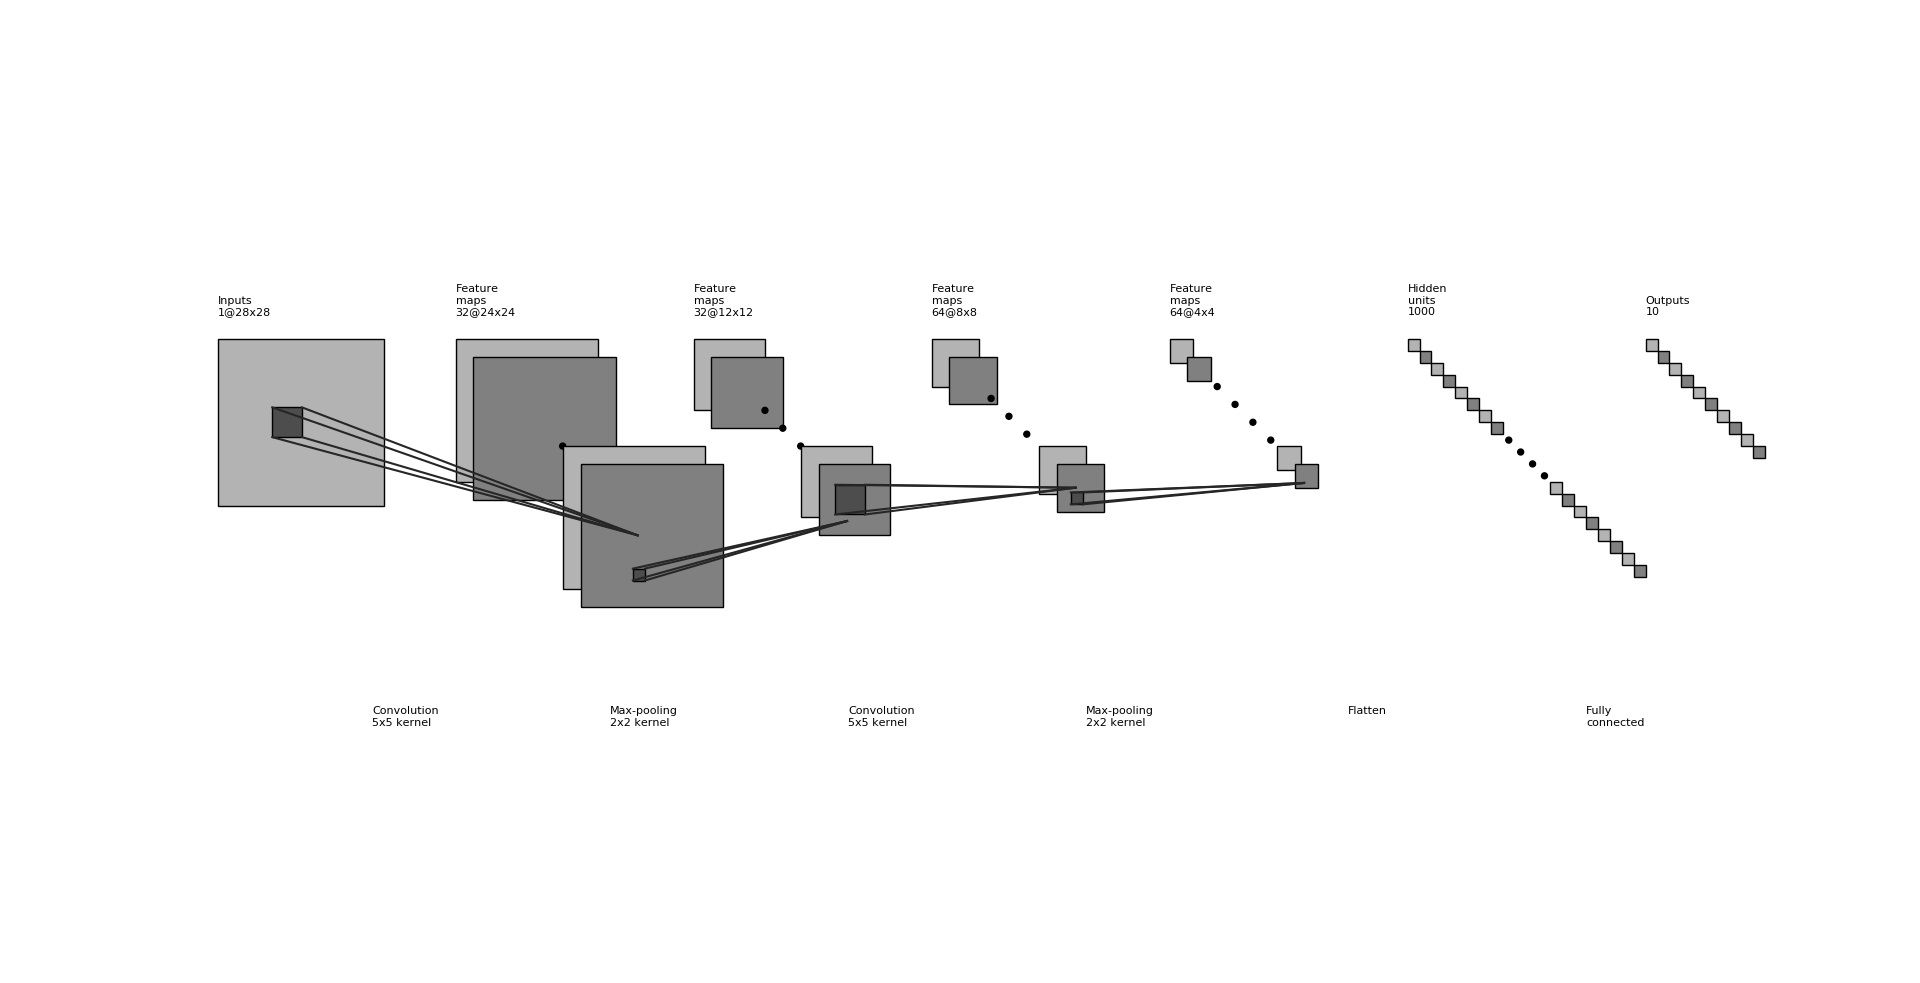
\includegraphics[width=\textwidth]{mnist}
\caption{\textbf{MNIST CNN Structure.} Two convolutional and max pooling layers followed by two fully connected layers resulting in a categorization for one of 10 handwritten digits.}
\centering
\end{figure}

\subsection{CIFAR-10/CIFAR-100}
The layout for the CIFAR-10 and CIFAR-100 dataset networks are very similar. For the CIFAR-10, we introduced dropouts to prevent overfitting. Other than dropouts and the number of convolutional/pooling layers the two networks are nearly identical. The CIFAR-100 network is the same as well however its filter sizes are slightly larger in each of the convolutional layers.

\section{Results}
During testing, the MNIST network was able to achieve a 99.7\% accuracy at best whereas the CIFAR-10 network maxed out at around 80\% and the CIFAR-100 at around 50\%. The CIFAR models were not trained nearly as much as the MNIST dataset due to the amount of time it took to train these two sets. Given more time they may have achieved around 90\% and 80\% accuracy respectively. In order to improve these results further, the network structure could be tested and altered based on which layer structures give the best results. Playing around with filters can also improve the network performance at cost of runtime.


\end{document}